
\section*{Background}

In deciding on the best method in which to portray scientific information we must first look at how our ability to understand comprehend information has changed over time. This section looks at now an increase in neocortex size proves pivotal to the sudden rise to power sapiens experinced as a species, and in turn the development of language and visualisation in the context of information transfer. 

In nature many animals are rely on the propagation of DNA to encode important information essential to their survival. Examples of these are seen in hives (where an insects role is defined by its genetic composition), or in Oscines (songbirds) which have an inherent predisposition to learn species specific songs, \cite{modelingpythonbees,genomics,birds,birdsongs,sapiens}.
In sapiens, the vast and varied nature of the information we are required to process makes this process highly impractical. Instead we develop a predisposition to learning language at an early age. Such a skill allows for the effective communication of ideas, conditions and dangers between a large number of people\footnote{Several studies, exploring the ratio of the neocortex to the rest of the brain, suggest that the number of relationships a human can successfully monitor is limited to ~150. It is suggested that ideas of gossip and common metaphysical beliefs are the reason for this \cite{sapiens,neo,gossip}. This limit is still seen in social networks today \cite{social}.}.

Howevever since communicatory patterns are limited to only the people they have been taught to, problems of differing language and dialect greatly reduce the amount of information which may be passed between groups or tribes. One way to overcome falls in the use of pictographs, a form of visualisation colloquially known as cave paintings (e.g. \autoref{cave}) which complements the sapien ability to both detect shapes and spot patterns within nature\footnote{It has been found that 10,000-year-old pictographs show hints of a common cultural background between spatially different groups of humans \cite{cave}.}. As communities increased in size, problems of accounting and resource management begin to emerge.




 \emph{REWRITE:
 Until this point an ability to store large amounts of numerical data had not been required by a hunter-gatherer species.} Around 3,500BC, the Samaritans solved this probelm with the creation of a system for coordinating affairs and storing information external to peoples brains. 

This system is that of writing \cite{archaic,beforeCuneiform}. Here quantities and items are depicted using a numerical system of signs and visual system of shapes (cuneiform\footnote{This is often mistaken for hieroglyphics. Although both are forms of logographic script, hieroglyphs are restricted to the ancient Egyptian sociolinguistic context. }). This external method of storing information, coupled with visual representation, allowed for a an effective and intuitive way for us to apply the pattern recognition and analytical parts of our brain whilst reducing the cognitive load by breaking up the problem into managable parts. 


\begin{figure}[H]
         \centering
         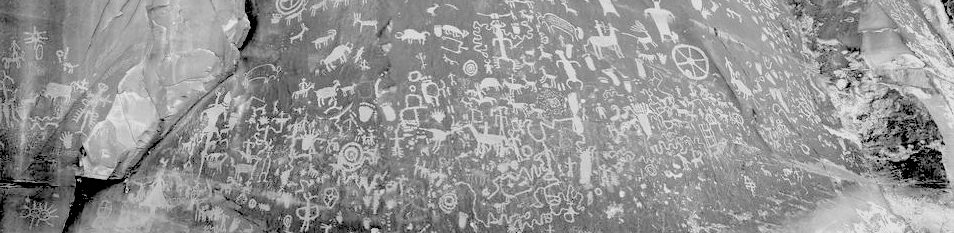
\includegraphics[width=\textwidth]{figures_c1/newspaperrock.jpg}
        \caption{\textbf{An example pictograph:} a 2000 year old petroglyth in Utah titled `Tse Hane' (rock that tells a story). Source:
        \cite{newspaperrock} }
        \label{cave}
\end{figure}

Throughout history, we have continued to apply this system of intertwining data information with visual artifacts to enable people to cope with the complexities of the infomation provided, \cite{tufte}. In the remainder of this chapter the use of visualisation as a means of enchancing the readers ability to understand the large-scale complexities of the chemistry within the troposphere shall be explored. 


\textbf{A note on terminology}
Although the word \emph{species} refers to the biological definition within this section, any further reference throughout this thesis refers to the chemical definition instead. 





%-----------------------------------------------
